
\newpage
\subsection{Analysis of g} % To be changed

With the definition of labor $L_t = (1-u_t)N^y_t$ and the definition of the labor share $\theta_t = \frac{w_t L_t}{Y_t} \Leftrightarrow \frac{1-\theta_t}{\theta_t} = \frac{Y_t}{w_t L_t} - 1$. Moreover, $X_t = \ln\left[\frac{(1-\tau_t)w_t}{b_t}\right]$. We obtain:
\begin{equation*}
X_t = \ln\left(\frac{\frac{u_t}{1-u_t}}{\eta_t\frac{1-\theta_t}{\theta_t}-1}\right)
\end{equation*}
We have that $\frac{u_t}{1-u_t} = \frac{N_t^y}{L_t} = \frac{N_t^y}{K_t}k_t$ and $\frac{1-\theta_t}{\theta_t} = \frac{\phi}{1-\phi}k_t^{\frac{\sigma-1}{\sigma}}$. Replacing in the previous equation,
\begin{equation*}
X_t = \ln \left( \frac{\frac{N_t^y}{K_t}k_t -1}{\frac{\phi}{1-\phi}k_t^{\frac{\sigma-1}{\sigma}}\eta_t -1} \right)
\end{equation*}
Let $X_t = g(k_t)$. Due to the logarithm, we have two vertical asymptotes depending on whether the numerator or the denominator within the logarithm is equal to zero. The first vertical asymptote is the one associated to the numerator: $k_1 = \frac{K_t}{N_t^y}$ and the second vertical asymptote is associated to the denominator: $k_2 = \left(\frac{1-\phi}{\phi} \frac{1}{\eta_t}\right)^{\frac{\sigma}{\sigma-1}}$. Rewriting the $g$ function with the vertical asymptote, we have:
\begin{equation*}
g(k_t) = \ln\left( \frac{\frac{k_t}{k_1}-1}{\left(\frac{k_t}{k_2}\right)^{\frac{\sigma - 1}{\sigma}} - 1} \right)
\end{equation*}
The function $g(k_t)$ has four different shapes according to the value of $\sigma$ and both vertical asymptotes ($k_1$ and $k_2$).\footnote{The function graphs are drawn using numerical computation with the following set of parameters for each case: a) $\sigma = 0.8$, $k_1 = 1$, $k_2 = 2$\\ b) $\sigma = 0.8$, $k_1 = 2$, $k_2 = 1$\\ c) $\sigma = 1.2$, $k_1 = 1$, $k_2 = 2$\\ d) $\sigma = 1.2$, $k_1 = 2$, $k_2 = 1$\\}


%\begin{figure}[ht] 
%	\begin{subfigure}[b]{0.5\linewidth}
%		\centering
%		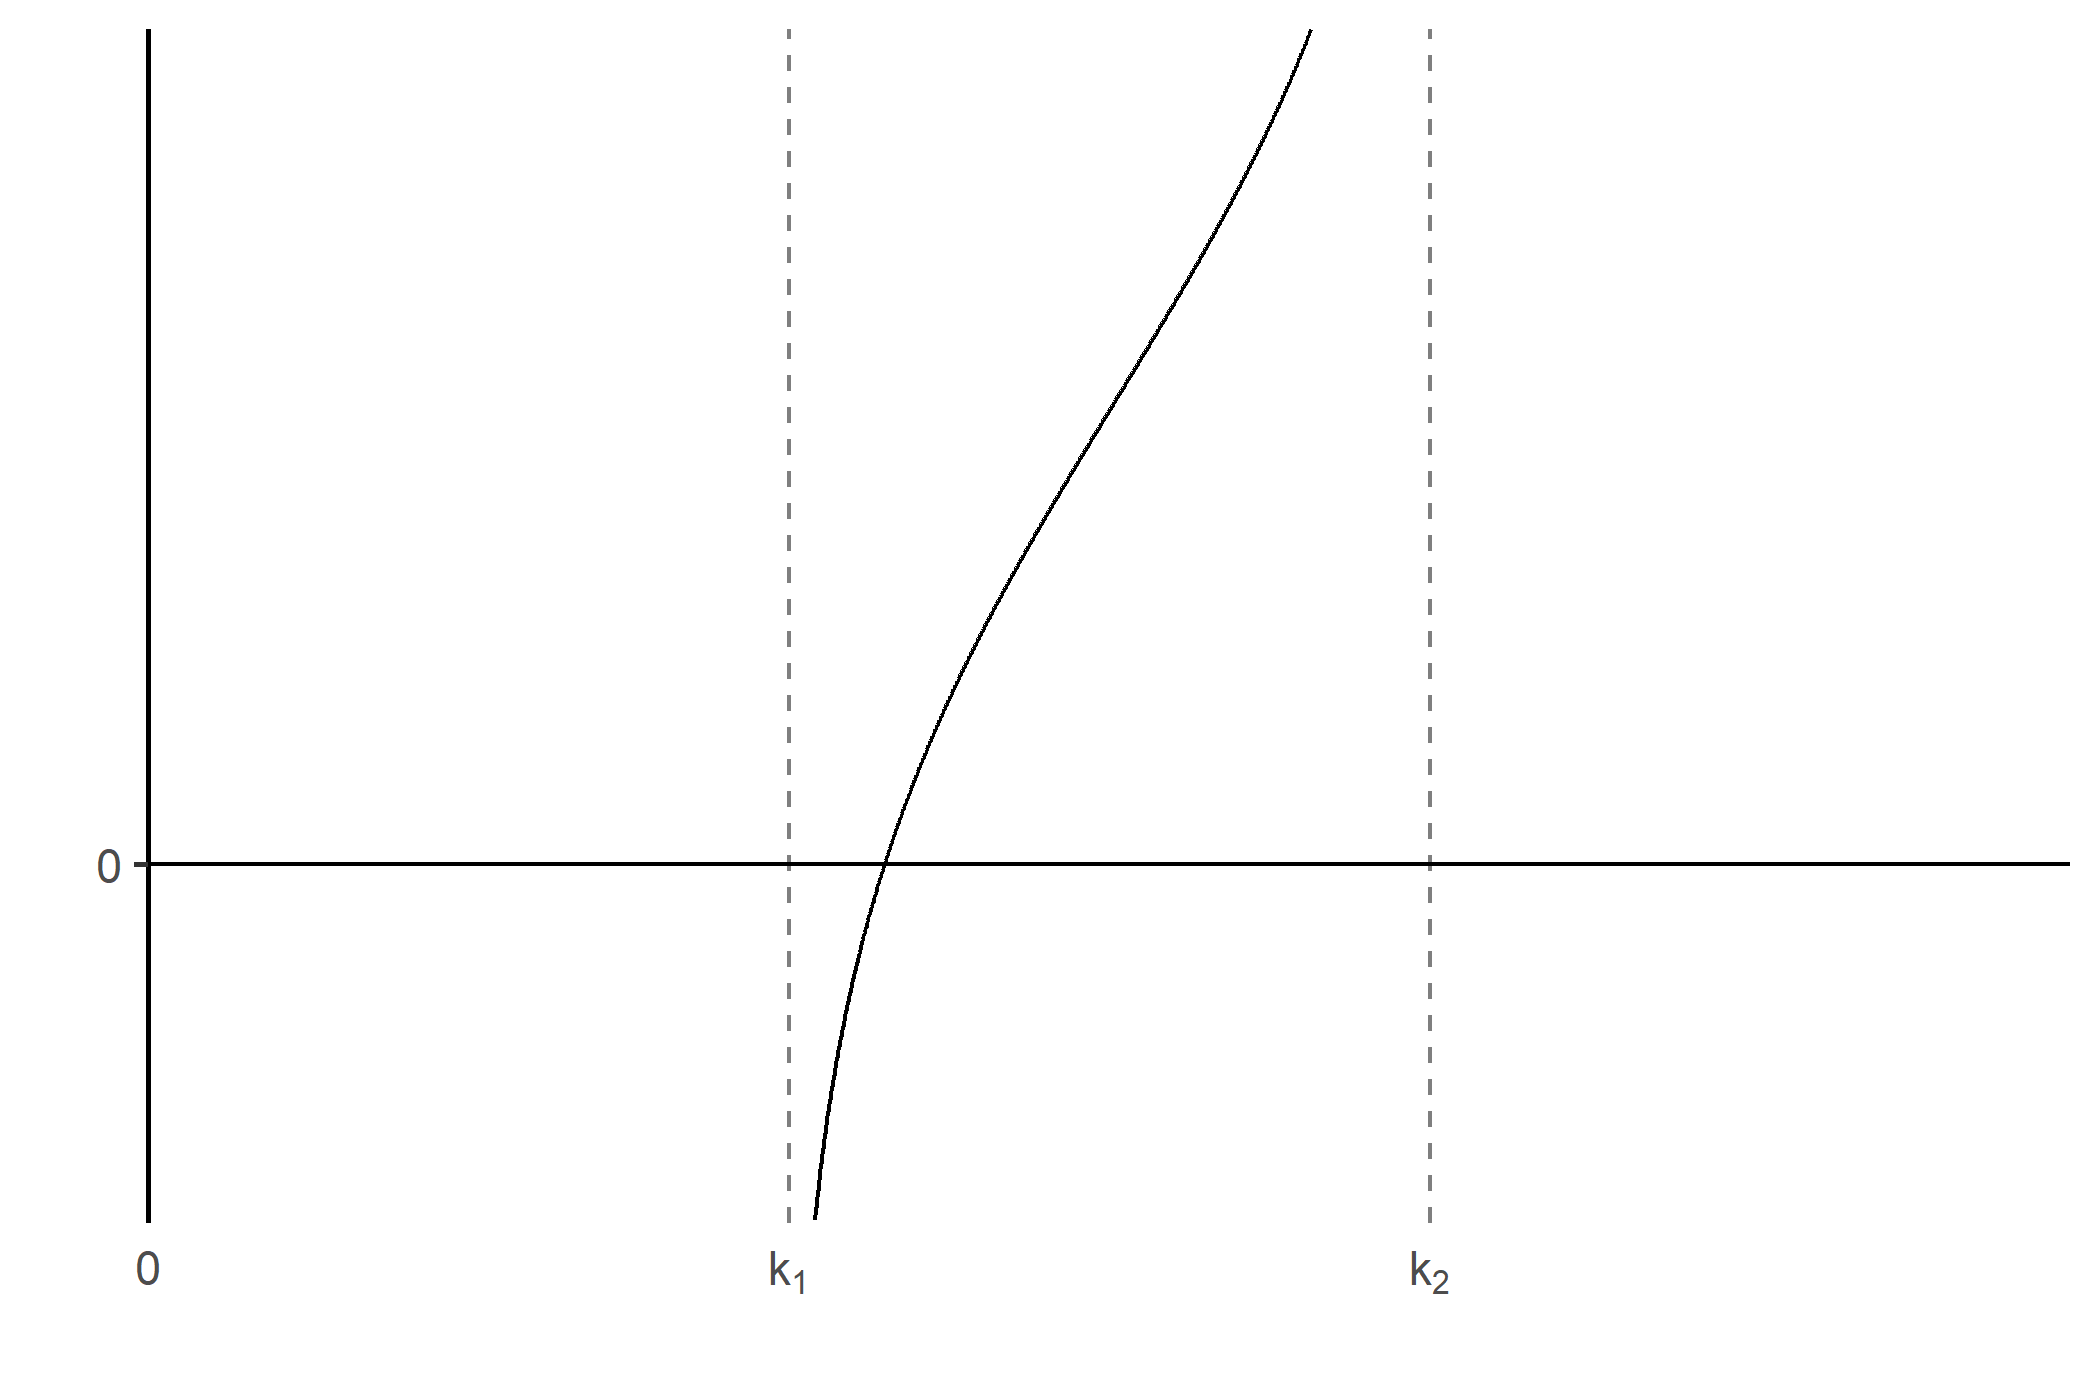
\includegraphics[width=1\linewidth]{Figures/graph_a} 
%		\caption{$\sigma = 0.8$, $k_1 = 1$, $k_2 = 2$} 
%		\label{fig:graph_a} 
%		\vspace{4ex}
%	\end{subfigure}
%	%%%
%	\begin{subfigure}[b]{0.5\linewidth}
%		\centering
%		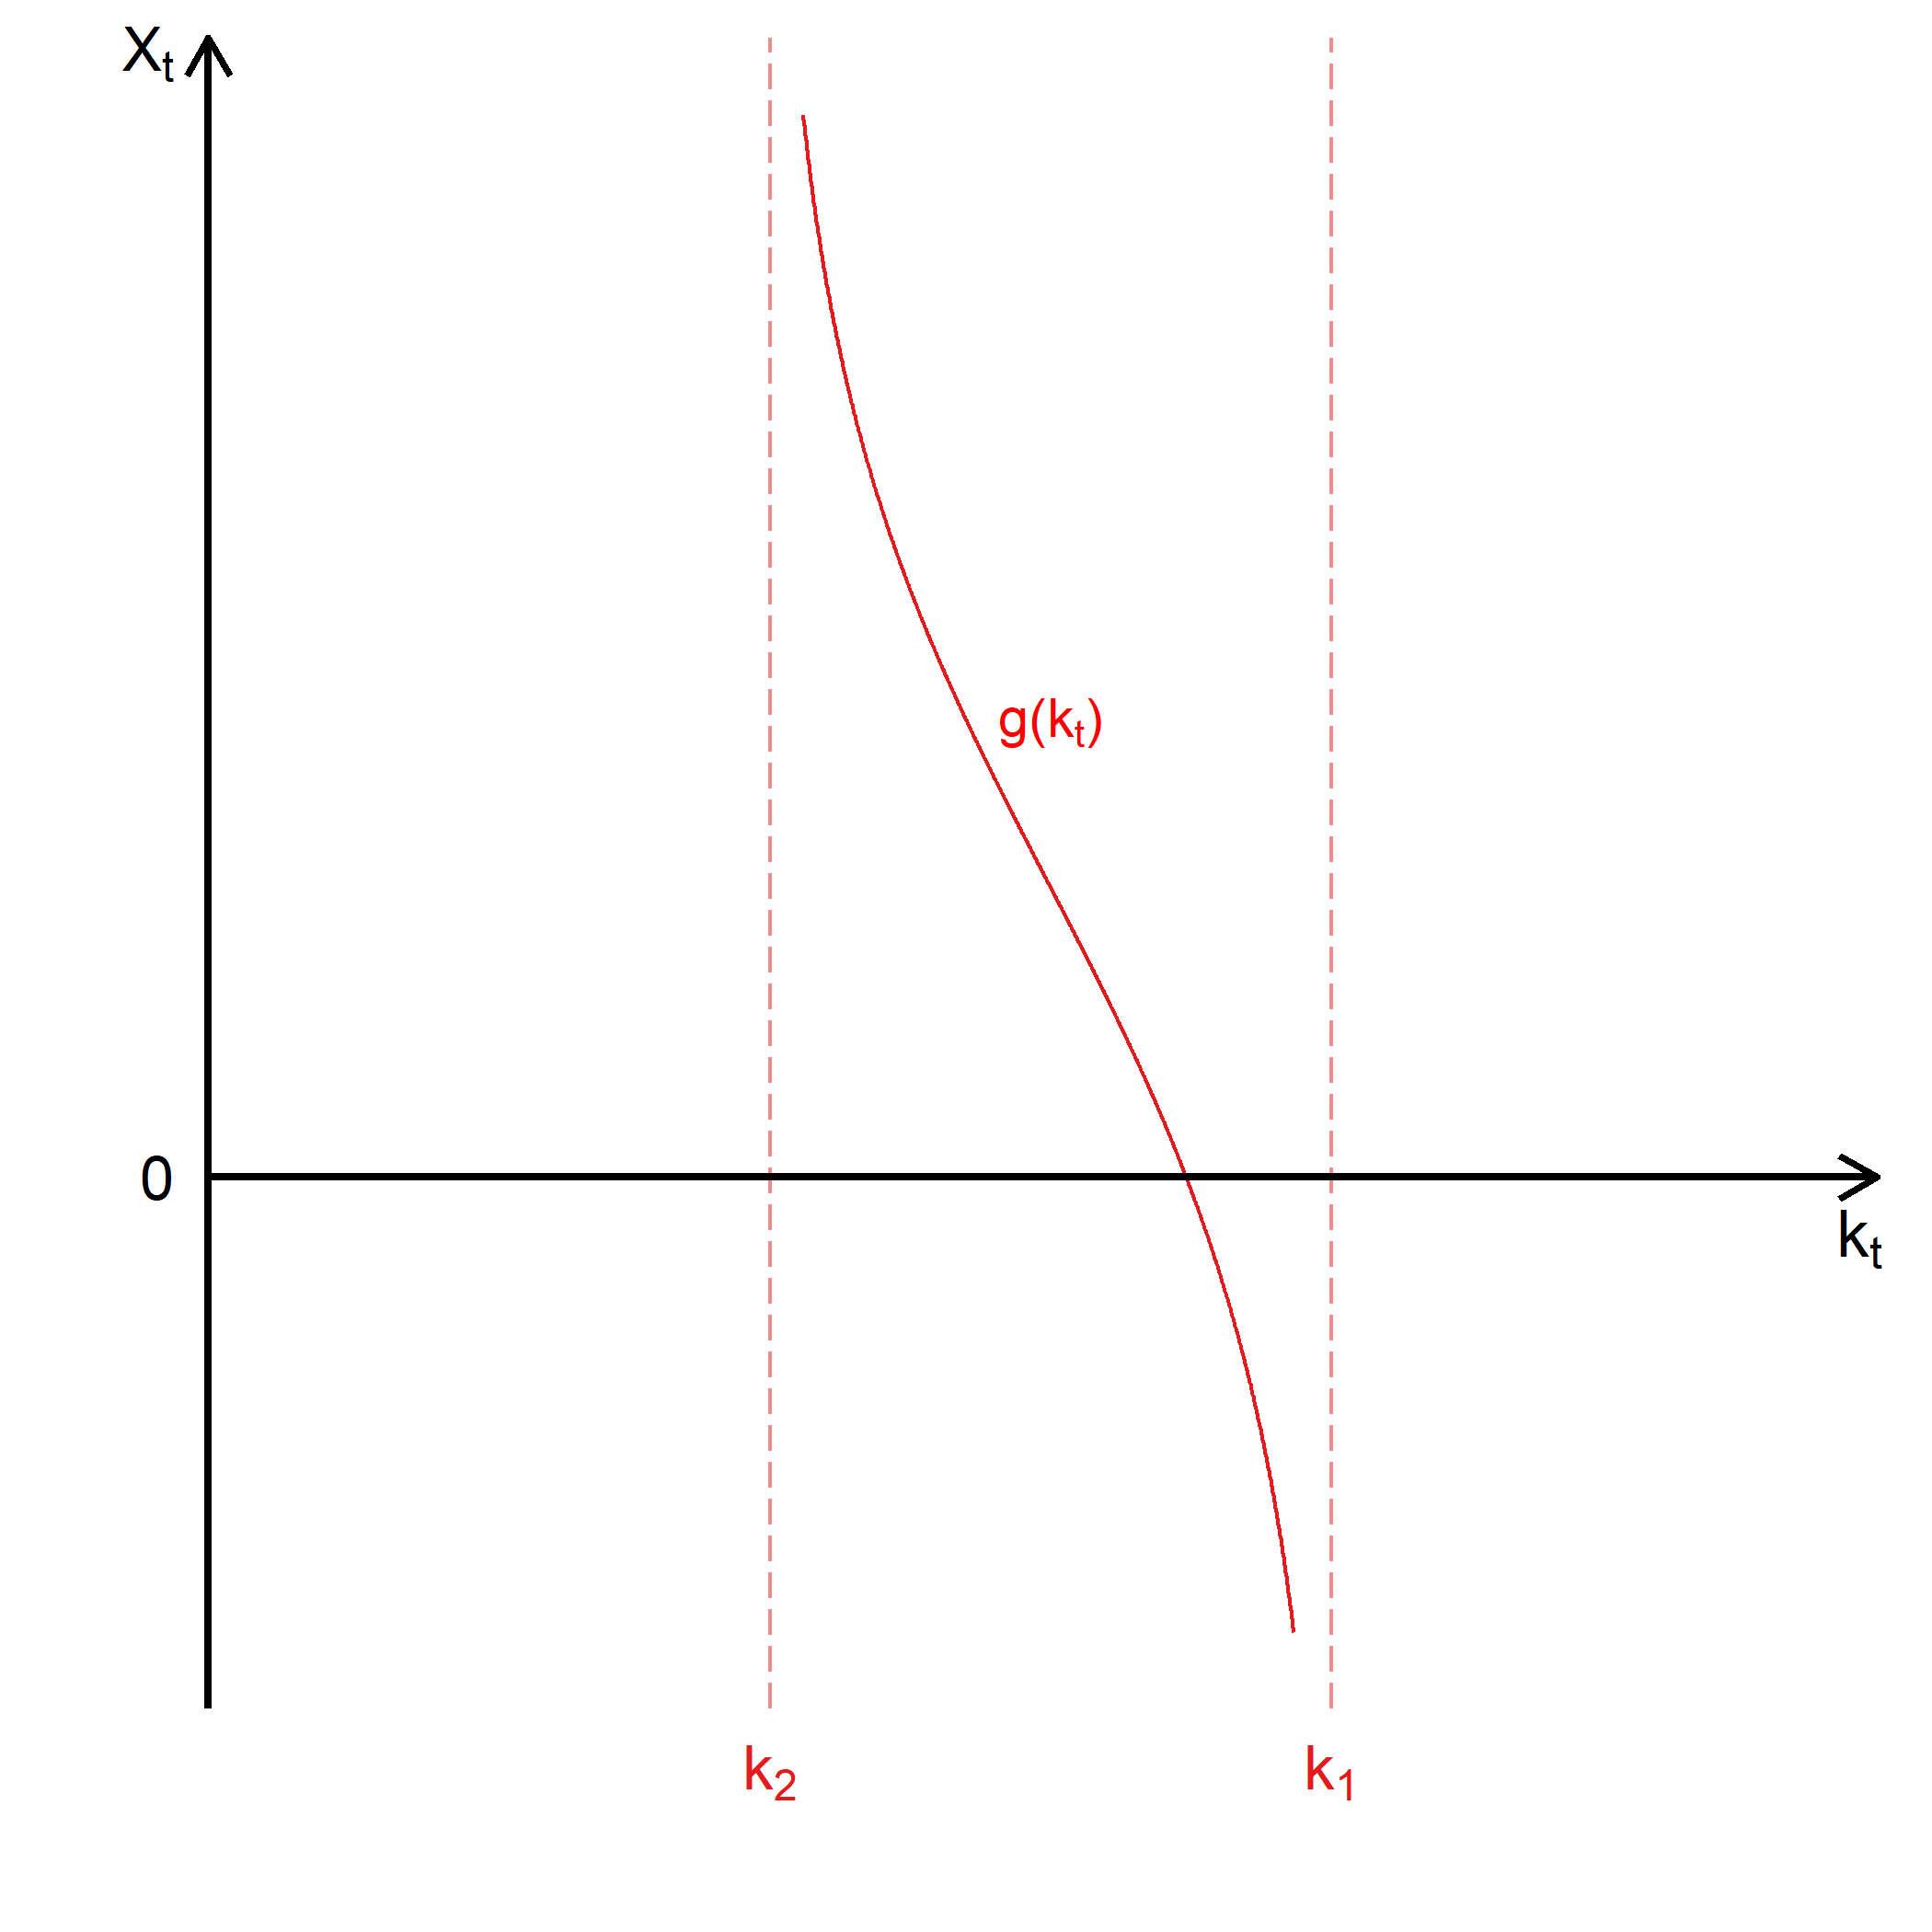
\includegraphics[width=1\linewidth]{Figures/graph_b} 
%		\caption{$\sigma = 0.8$, $k_1 = 2$, $k_2 = 1$} 
%		\label{fig:graph_b} 
%		\vspace{4ex}
%	\end{subfigure}
%	%%%
%	\begin{subfigure}[b]{0.5\linewidth}
%		\centering
%		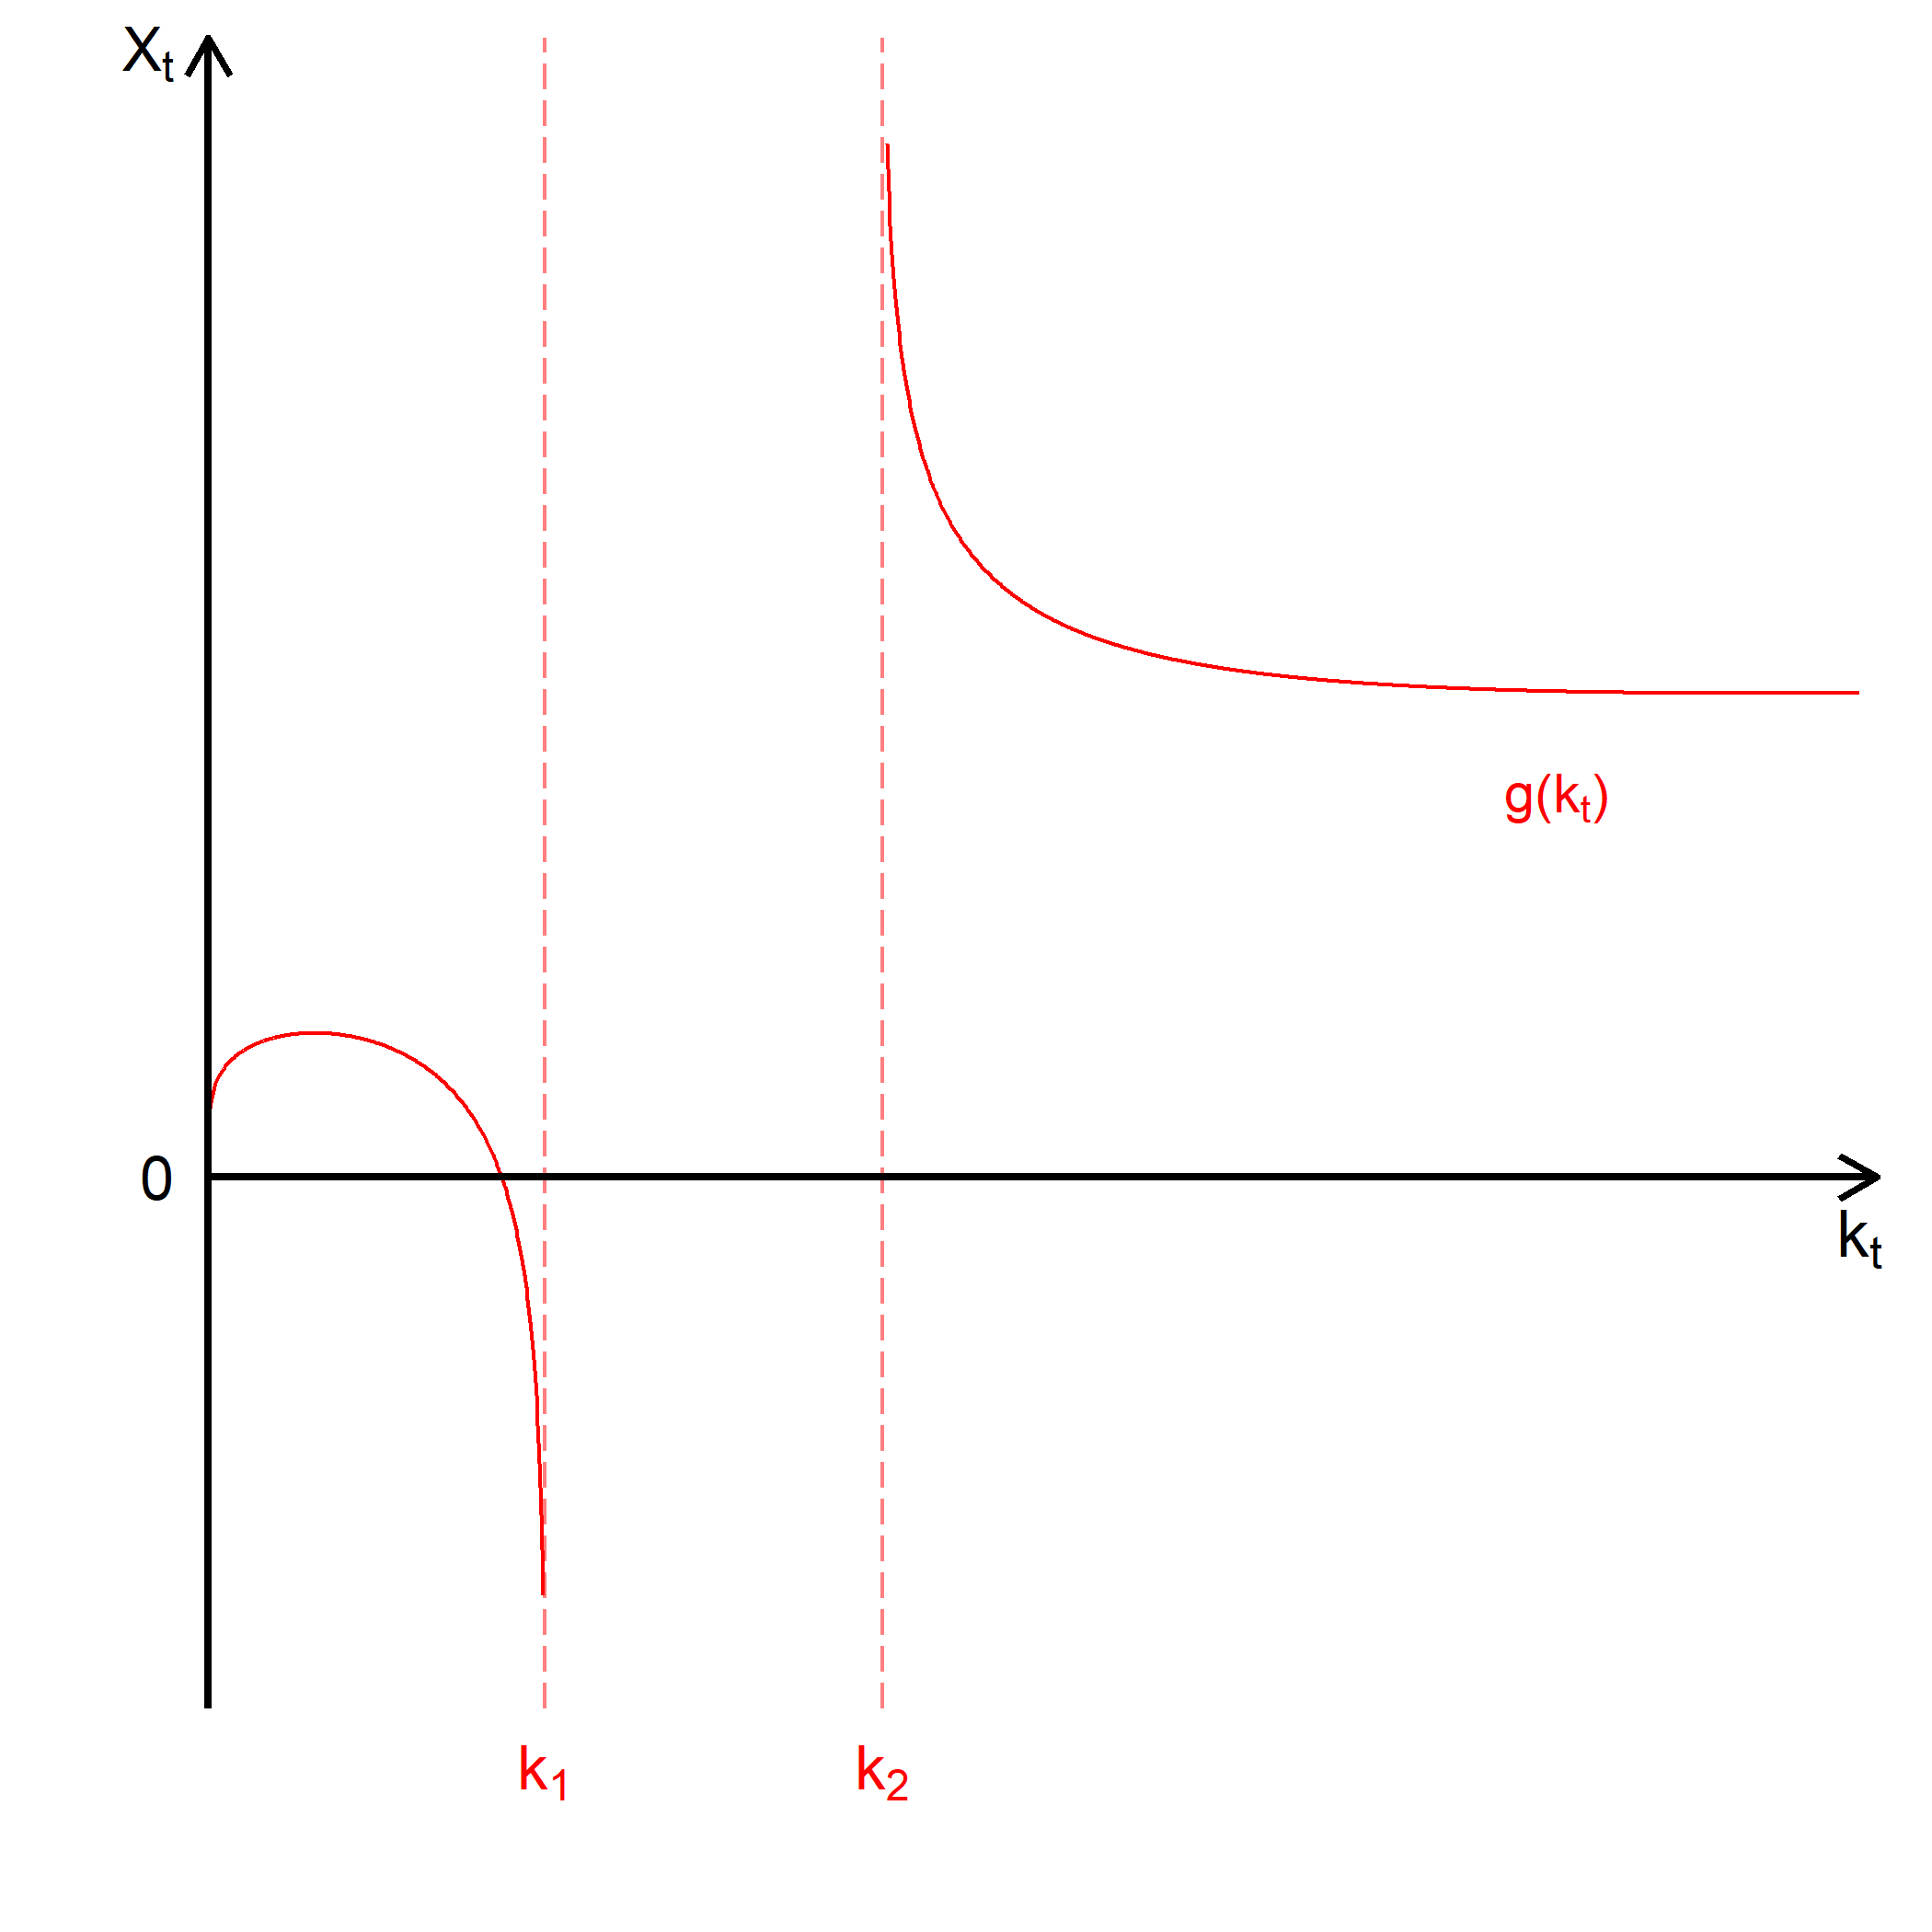
\includegraphics[width=1\linewidth]{Figures/graph_c} 
%		\caption{$\sigma = 1.2$, $k_1 = 1$, $k_2 = 2$} 
%		\label{fig:graph_c} 
%	\end{subfigure}
%	%%%
%	\begin{subfigure}[b]{0.5\linewidth}
%		\centering
%		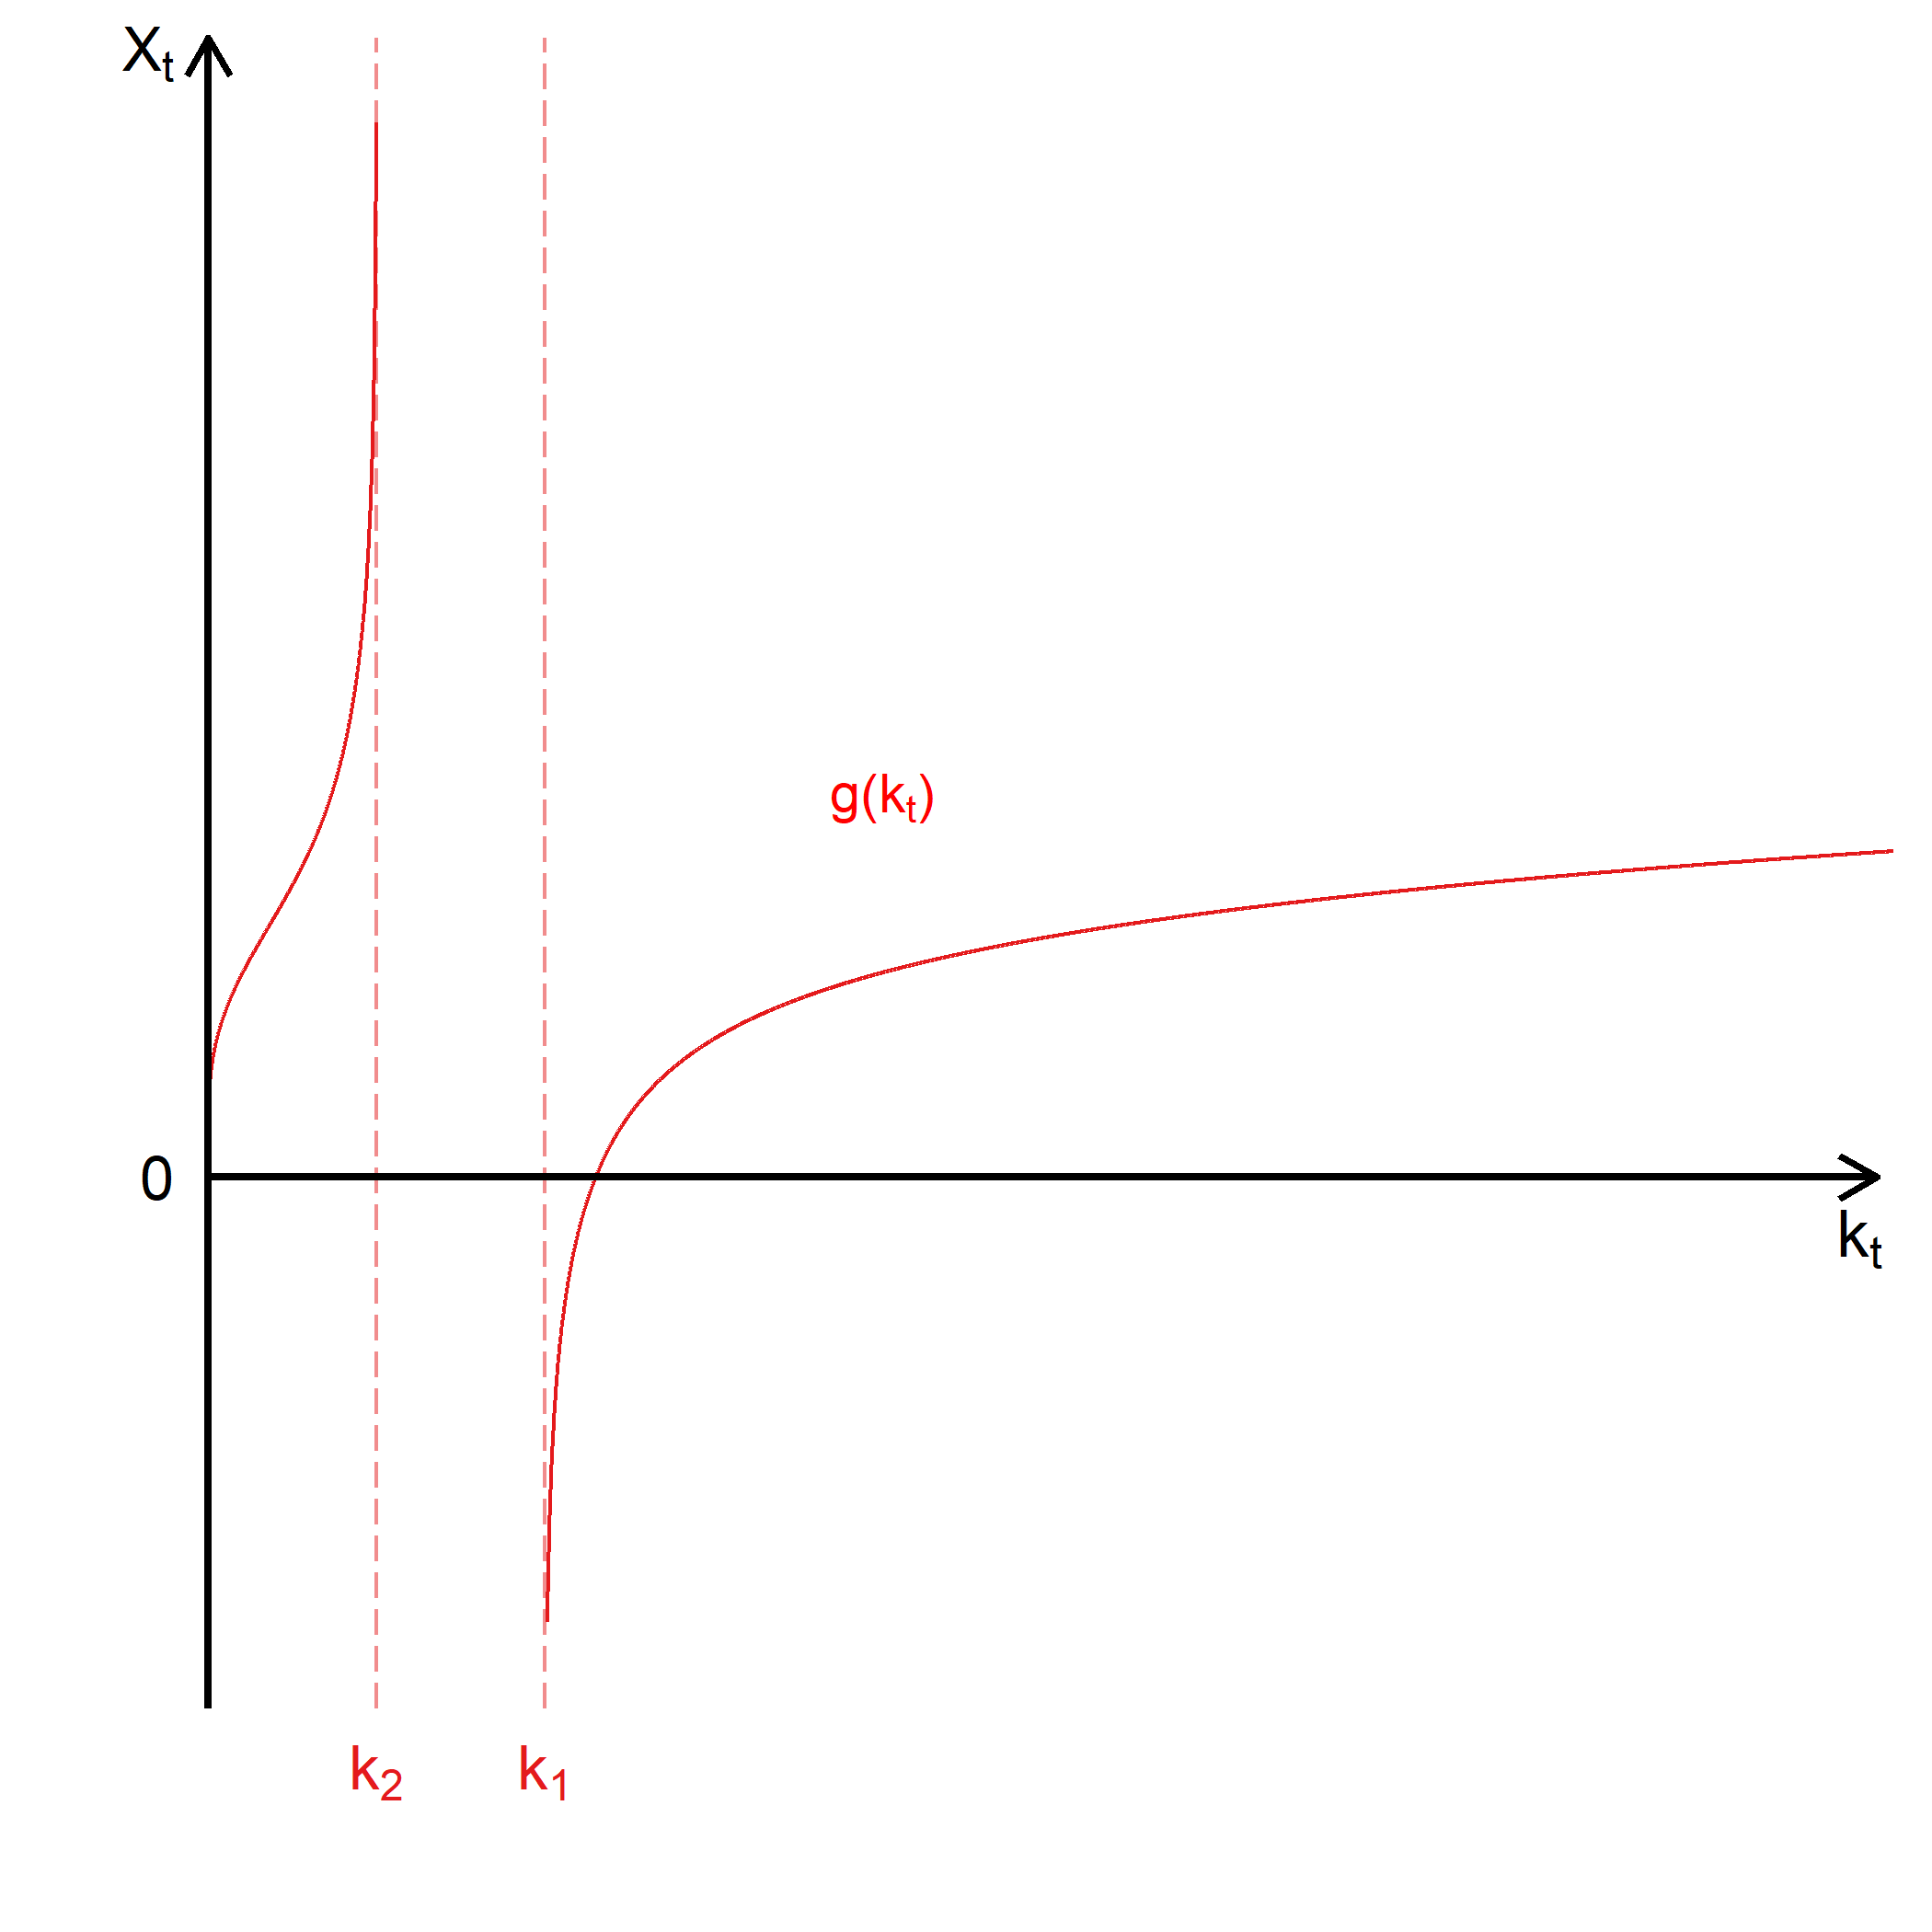
\includegraphics[width=1\linewidth]{Figures/graph_d} 
%		\caption{$\sigma = 1.2$, $k_1 = 2$, $k_2 = 1$} 
%		\label{fig:graph_d} 
%	\end{subfigure} 
%	\caption{Different possible shapes of the $g$ function}
%	\label{fig:g_shape} 
%\end{figure}
%
%
%\begin{figure}[ht] 
%	\begin{subfigure}[t]{0.5\linewidth}
%		\centering
%		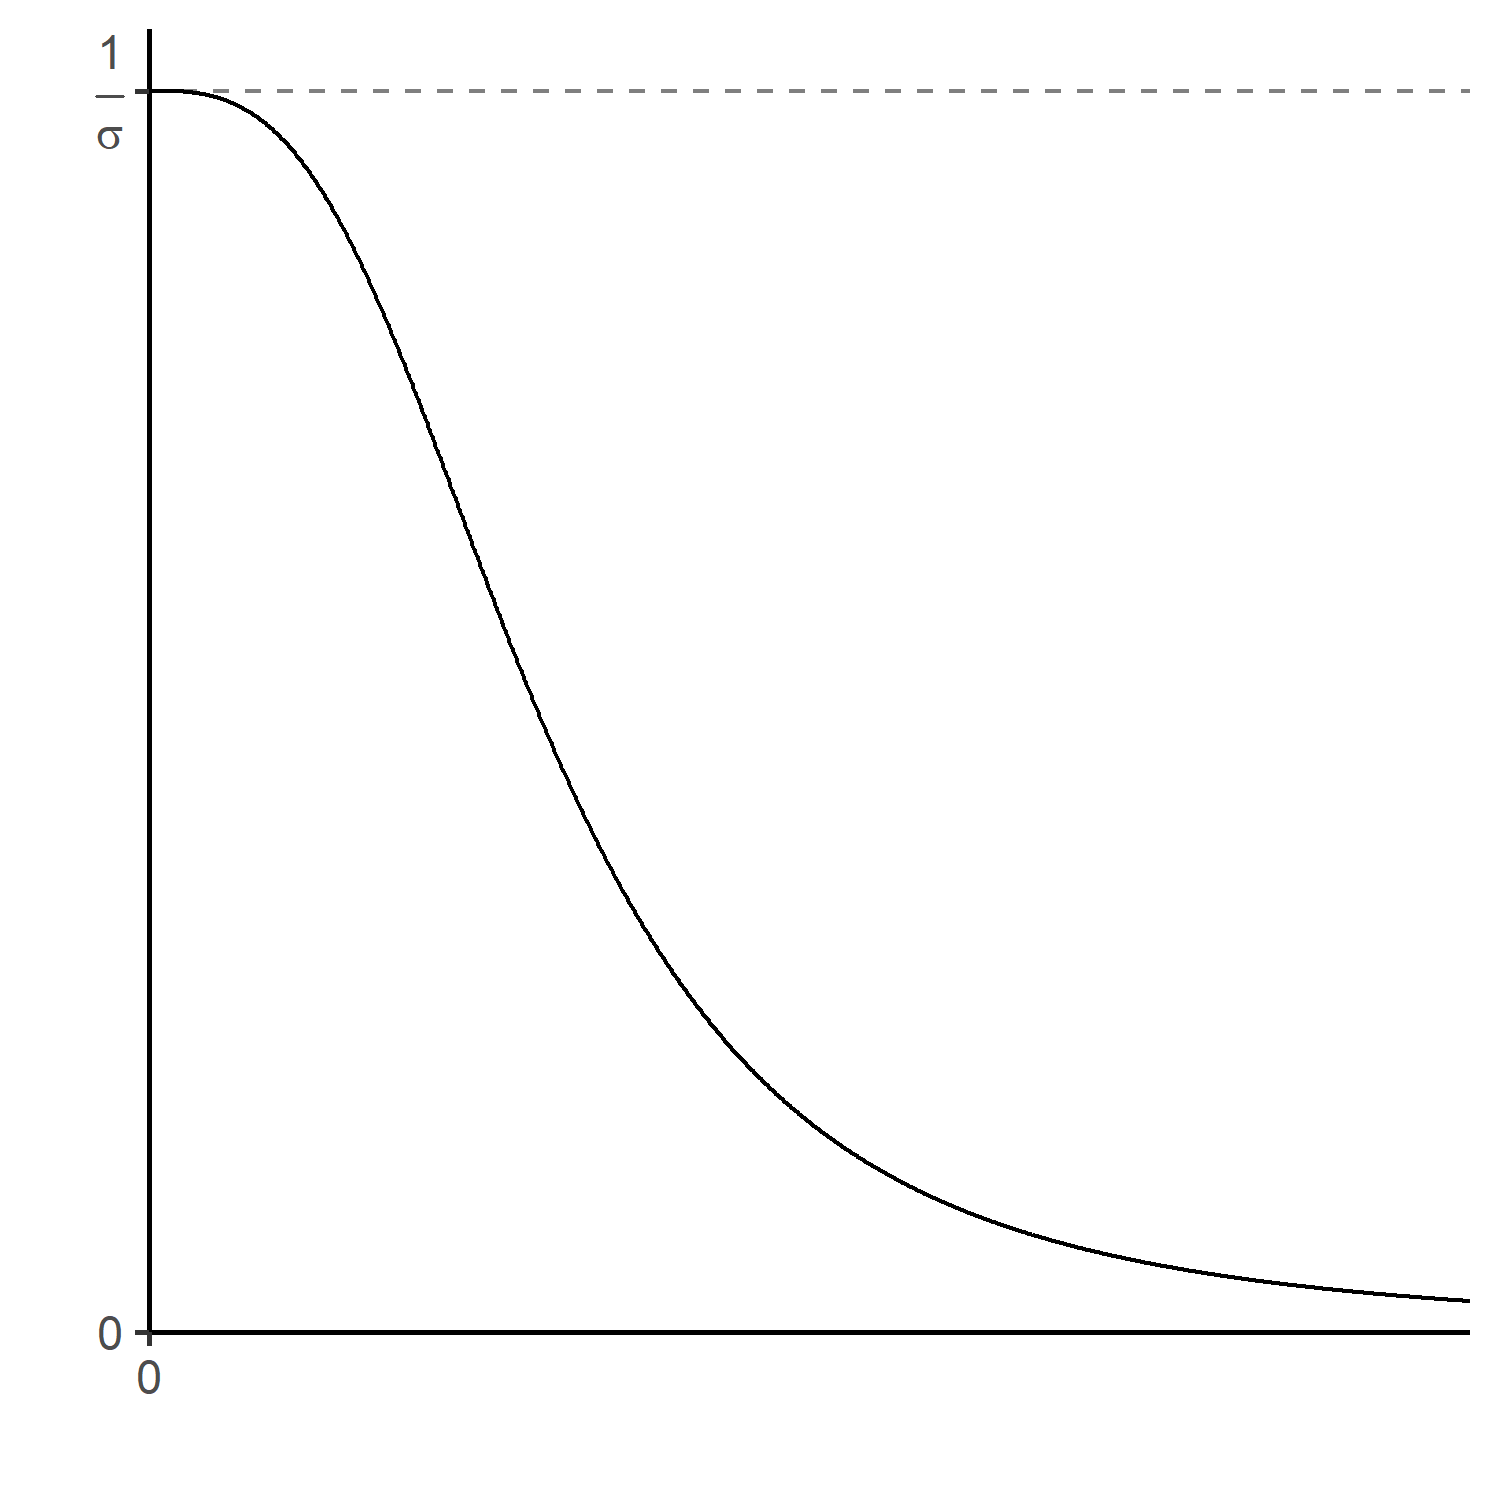
\includegraphics[width=1\linewidth]{Figures/graph_1} 
%		\caption{$\sigma = 0.25$, $\phi = 0.3$, $\gamma = 0.5$} 
%		\label{fig:graph_1} 
%		\vspace{4ex}
%	\end{subfigure}
%	%%%
%	\begin{subfigure}[t]{0.5\linewidth}
%		\centering
%		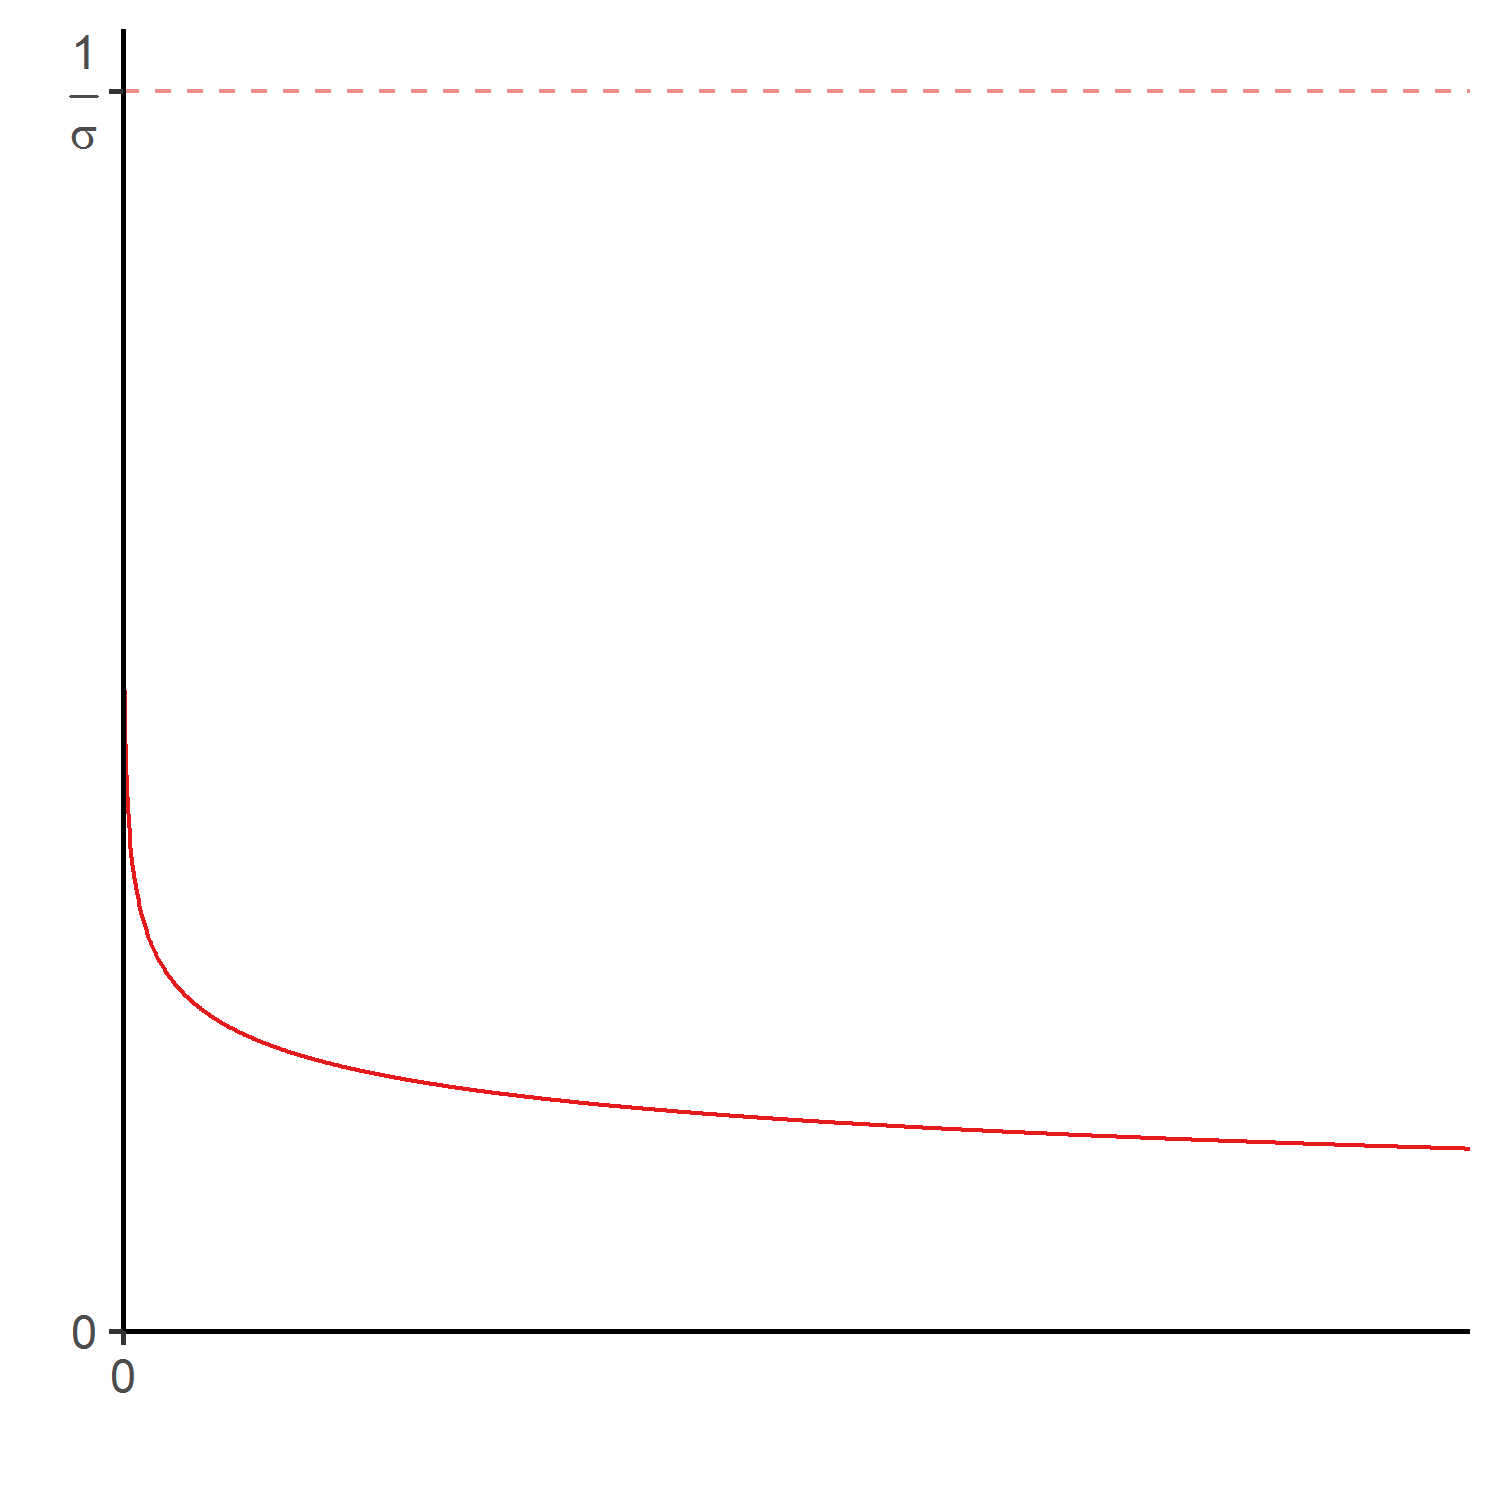
\includegraphics[width=1\linewidth]{Figures/graph_2} 
%		\caption{$\sigma = 0.8$, $\phi = 0.3$, $\gamma = 0.5$} 
%		\label{fig:graph_2} 
%	\end{subfigure}
%	%%%
%	\begin{subfigure}[t]{0.5\linewidth}
%		\centering
%		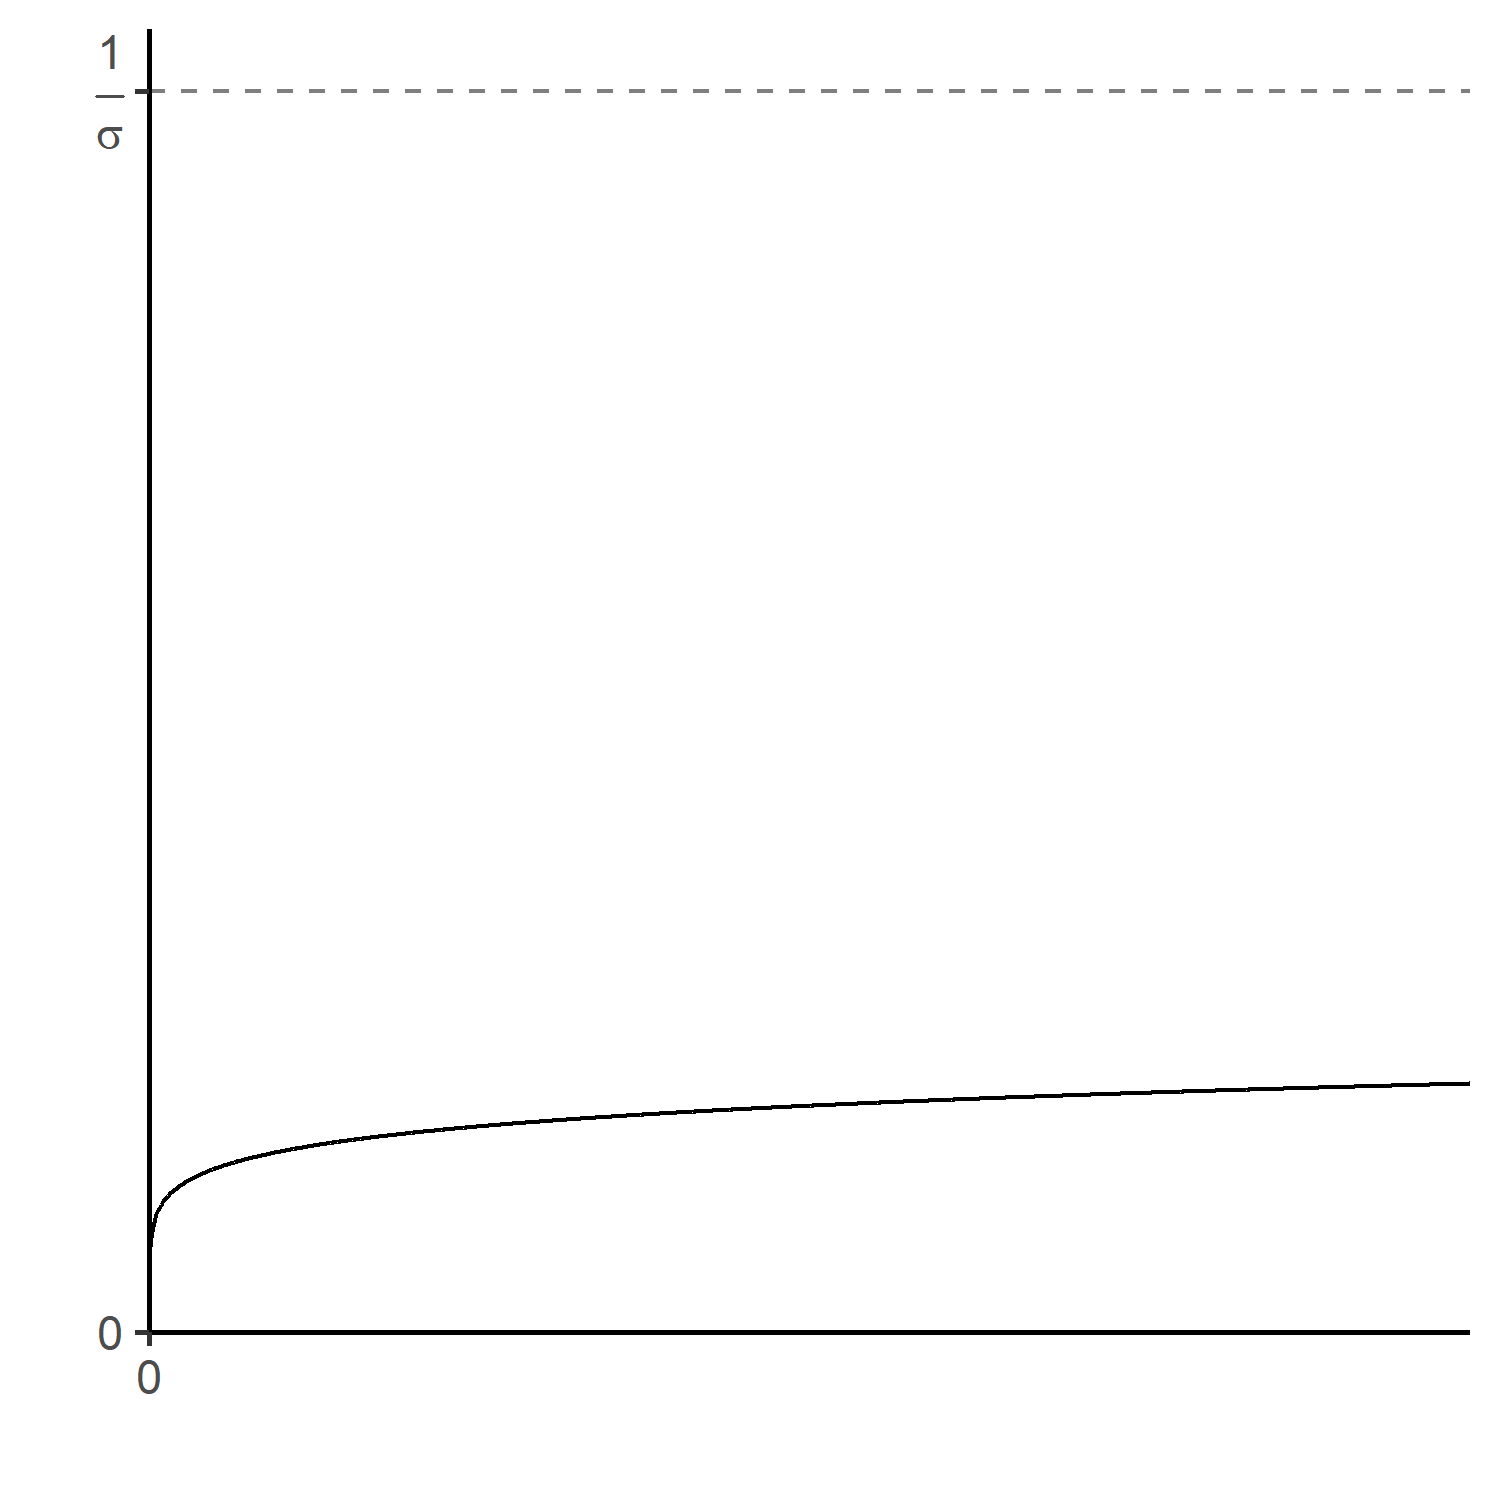
\includegraphics[width=1\linewidth]{Figures/graph_3} 
%		\caption{$\sigma = 1.2$, $\phi = 0.3$, $\gamma = 0.5$} 
%		\label{fig:graph_3} 
%	\end{subfigure} 
%	\caption{Different possible shapes of the $h$ function}
%	\label{fig:h_shape} 
%\end{figure}







Focusing on the first vertical asymptote, $\frac{N_t^y}{K_t}k_t -1 > 0 \Leftrightarrow k_t > k_1 \Leftrightarrow L_t < N_t^y$. It means that the numerator is positive if and only if the capital per worker is greater than the capital per young individual (i.e. the number of worker is smaller than the young population size). Since there is unemployment, this condition is always satisfied. Thus, $k_t > k_1$.




